\documentclass{../notatki}

\title{Wstęp do Fizyki Kwantowej}

\begin{document}

\section{Wstęp}

$$
E^2 =c^2p^2 + m^2c^4
$$

\section{Eksperyment Younga}

W eksperymencie mierzymy zachowanie elektronów względem
dwóch dziur i czujnika ruchomego na wzdłuż osi $x$. Mierzymy prawdopodobieństwo,
tego, że czujnik odbierze elektron, jako $P_{12}(x)$. Równocześnie rozróżniamy
$P_1(x)$ oraz $P_2(x)$; prawdopodobieństwa, tego, że czujnik odbierze
elektron przy jednej z dziur zasłoniętej.

\begin{figure}[H]
  \centering
  \begin{tikzpicture}
    \node[draw] (source) at (-4,2) {źródło};

    \draw (0,0) -- (0, 1.8);
    \draw (0, 2) -- (0, 2.3);
    \draw (0, 2.5) -- (0,4);

    \draw[thick] (2,0) -- (2,4) node[above] {$x$};

    \draw[->] (source.east) -- (0, 2.4);
    \draw[->] (source.east) -- (0, 1.9);

  \end{tikzpicture}
  \caption{Ilustracja eksperymentu}
\end{figure}

\subsection{Cząstkowa interpretacja}

Jeśli elektron zachowałby się jako cząstka, to spodziewalibyśmy się, że
$P_{12}(x) = P_1(x) + P_2(x)$. Wnioskiem takiej obserwacji byłoby, że
cząstki elektronów nie mają na siebie wpływu; nie zachodzi interferencja.
Co więcej, elektron zawsze przechodzi jedną dziurą.

\subsection{Falowa interpretacja}

Jeśli elektron zachowałby się jako fala, to spodziewalibyśmy się
przeciwnego wyniku. Fale nie nakładają się na siebie tak czysto.
Zachodziłaby interferencja; fale w zależności od fazy albo by się na siebie
nakładały, albo niwelowały. Co więcej ze wzlędu na działanie fal, elektron
by przechodził przez obydwie dziury jednocześnie.
$P_{12}(x) = |\phi_1(x) + \phi_2(x)|^2$,
$P_1 = |\phi_1(x)|^2$, \dots.

\subsection{Wynik}

Eksperyment pokazuje, że mimo tego, że detektor odbiera elektrony
w dyskretnych grupach, to $P_{12}$ zachowuje się jakby elektrony były falami.
Zatem elektron zachowuje się "trochę jak cząstka trochę jak fala".

Dodanie źródła światła do eksperymentu, co pozwala nam go zobaczyć, powoduje, że
elektrony zachowują się jak cząstki. Wynika to z tego, że światło wpływa na
elektrony.

Na podstawie tego eksperymentu, opracowano zasadę niepewności Heisenberga.
W ramach eksperymentu, oznacza ona, że nie da się zaprojektować detektora
elektronów, który nie wpływa na elektrony.

\subsection{Wyprowadzenia}

Ten eksperyment pozwala nam wyprowadzić następujące właściwości
światła o danej długości fali $\lambda$ i częstości $\omega$:

$$
k = \frac{2 \pi}{\lambda}
$$
$$
p = \frac{2\pi\hbar}{\lambda} = \frac{h}{\lambda} = k\hbar
$$
$$
E_f = \hbar \omega = pc
$$
Zatem też: $m_f = 0$, $v_f = c$.

\subsection{Światło}

\noindent \textit{Światło o danym $\lambda$ i $\omega$ składa się z
dyskretnych cząstek, których dystrybucja jest dana przez interferencję fali}.
Nie jest falą, ale działa jak fala. Charakterystyka fali określa
prawdopodobieństo, tego że foton padnie w danym miejscu.

\subsection{Fala de Broglie}

Jest to generalizacja koncepcji światła wychodzącej z eksperymentu Younga.
Każda fala, która na skali makroskopicznej zachowuje się jak fala, lecz tak
naprawdę jest masą dyskretnych cząstek jest falą de Broglie, lub falą materii.

$$
\lambda = \frac{h}{p}
$$
$$
E = h\nu
$$

\section{Zasada niepewności}

$$
\Delta x \Delta p \geq \frac{\hbar}{2}
$$
gdzie, na przykład, $\Delta x = \sigma(x)$. Istotna jest jednak obserwacja, że
dla $\Delta x \rightarrow 0$, $\Delta p \rightarrow \infty$, i na odwrót.

\section{Efekt Fotoelektryczny}

W wyniku promieniowania fotonami, elektrony atomów pierwiastka są
wyrzucane z atomu. Efekt ten jest wykorzystywany w praktyce w
napędzaniu fotodiod i fotokomórek.

Elektrony w metalu znajdują się w studni potencjału, głębokości $W$,
odpowiadającej pracy wyjścia.
Foton padając na materiał powoduje wyrzucenie elektronu naładowanego
$U$ z energią kinetyczną $E_{k \text{max}}$. W wyniku tego procesu
utracona zostaje energia w postaci pracy wyjścia $W$:
$$
E_{k \text{max}} = E_f - W = eU
$$
Częstością progową nazywamy najniższą częstość $\omega_0$, dla której
$E_{k \text{max}} = 0$.

\section{Zjawisko Comptona}

W zjawisku Comptona foton padający na elektron zmienia kierunek i
częstość. Efekt ten jest wykorzystywany w praktyce w analizie struktury
atomów i molekuł.

\begin{figure}[H]
  \centering
  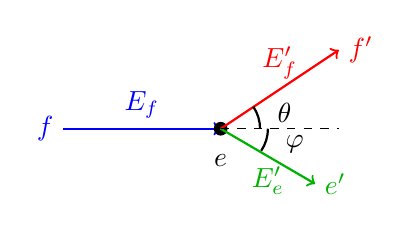
\begin{tikzpicture}
    \draw[->,thick,blue] (-2,0) -- (0,0) node[midway,above] {$E_f$};
    \draw[blue] (-2,0) node[left] {$f$};

    \draw[fill=black] (0,0) circle (0.08);
    \draw (0,-0.2) node[below] {$e$};

    \draw[->,thick,red] (0,0) -- (1.5,1) node[midway,above] {$E_f'$};
    \draw[red] (1.5,1) node[right] {$f'$};

    \draw[->,thick,green!70!black] (0,0) -- (1.2,-0.7)
    node[midway,below] {$E_e'$};
    \draw[green!70!black] (1.2,-0.7) node[right] {$e'$};

    \draw[thick] (0.5,0) arc (0:34:0.5);
    \draw (0.6,0.2) node[right] {$\theta$};

    \draw[thick] (0.6,0) arc (0:-34:0.5);
    \draw (0.7,-0.2) node[right] {$\varphi$};

    \draw[dashed] (0,0) -- (1.5,0);
  \end{tikzpicture}
  \caption{Ilustracja zjawiska Comptona. Foton $f$ ma długość fali $\lambda$.}
\end{figure}

W zjawisku zachowanny jest pęd oraz energia, co wraz z równaniem Comptona:
$$
(\lambda' - \lambda) \frac{m_ec}{h} = 1 - \cos\theta
$$
Pozwala nam w istocie wyprowadzić wszystkie niewadome w zjawisku.

$$
p = \frac{h}{\lambda}
$$

$$
p_f + p_e = p_f' + p_e' \Rightarrow
\begin{cases}
  \frac{h}{\lambda} = \frac{h}{\lambda'}\cos\theta + p_e\cos\varphi \\
  0 = \frac{h}{\lambda'}\sin\theta + p_e\sin\varphi
\end{cases}
$$

$$
E_f + E_e = E_f' + E_e' \Rightarrow \frac{hc}{\lambda} + m_ec^2 =
\frac{hc}{\lambda'} + E_e'
$$

\section{Model Bohra}

W modelu atomu Bohra, elektron porusza się wokół jądra wokół jednej z
dyskretnych
orbit. To też oznacza, że energia elektronu jest dyskretna lub zkwantowana.

\begin{figure}[H]
  \centering
  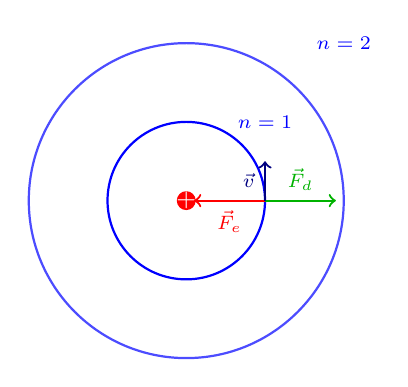
\begin{tikzpicture}
    \fill[red] (0,0) circle (0.12) node[white] {\small +};

    \draw[thick,blue] (0,0) circle (1);
    \draw[thick,blue,opacity=0.7] (0,0) circle (2);

    \node[blue] at (1,1) {\scriptsize $n=1$};
    \node[blue] at (2,2) {\scriptsize $n=2$};

    \draw[->,thick,green!70!black] (1,0) -- (1.9,0)
    node[midway,above] {\scriptsize $\vec{F}_d$};

    \draw[->,thick,red] (1,0) -- (0.1,0)
    node[midway,below] {\scriptsize $\vec{F}_e$};

    \draw[->,thick,blue!50!black] (1,0) -- (1,0.5)
    node[midway,left] {\scriptsize $\vec{v}$};

  \end{tikzpicture}
  \caption{Model Bohra atomu}
\end{figure}

Elektron na orbicie utrzymuje się w wyniku siły elektrostatycznej między
elektronem a jądrem.
$$
\frac{mv^2}{r} = k \frac{e^2}{r^2}
$$
$$
mvr = n\hbar = n\frac{h}{2\pi}
$$
Dla dowolnego ciała na orbicie:
$$
v = \frac{2\pi r}{T}
$$
gdzie $T$ jest czasem okresu orbity.
$$
E_k = - \frac{E_p}{2}
$$
Postulat Bohra:
$$
\oint pdq = nh
$$

\end{document}
